No Brasil há uma grande diversidade de redes fluviais que são dividida em regiões hidrográficas, uma dessas regiões é a Bacia Amazônica, considerada a mais extensa do mundo \cite{portalbrasil:2009}. As águas dessa bacia são classificadas em branca, preta e clara \cite{sioli:2012}. Segundo \citeonline{barthem:2004} os rios de água branca tem turbidez elevada dificultando a visibilidade dentro \textcolor{red}{da água}. De acordo com \citeonline{santos:2005} essa coloração branca é causada pela riqueza de minerais na água, e frequentemente entrada nos rios da região norte do Brasil.

Nos últimos anos a demanda pela identificação de objetos submersos têm crescido, dado ao grande avanço nas observações oceânicas, que resultam em grandes quantidades de dados visuais de ambientes submersos a serem processados. Espécies de peixes e população são as tarefas mais importantes na observação oceânica, beneficiando pesquisadores, como cientistas e biólogos, bem como aplicações comercias como piscicultura (Qin\todo{Corrigir está citação utilizando cite} et al 2016). 

Em aplicações para identificação de peixes, câmeras colocadas em redes de observação oceânicas enfrentam dificuldades extremas causadas pelos ambientes naturais, tal como atenuação da luz e recifes e corais. Segundo Qin\todo{Corrigir está citação utilizando cite} et al. (2016), com a utilização de matriz de decomposição para processar os vídeos, é possível extrair as linhas dos peixes em primeiro plano, assim eliminando o fundo da imagem, facilitando o processo de reconhecimento dos peixes.

Segundo Van\todo{Corrigir está citação utilizando cite} Damme (2015) é possível fazer a captação de dados em ambientes submersos, utilizando técnicas elementares como desenhos em escala, trilateração de fita métrica, medidas de deslocamento e fotografia simples. Esses métodos são ideais para fazer reconhecimento de sítios arqueológicos submersos. Porém esses métodos não são precisos, com exceção da fotografia, e levam muito tempo para serem construídos, e são propensos a erros humanos. Essas técnicas produzem apenas representações bidimensionais e tridimensionais com baixo nível de detalhes do local estudado.

Segundo  Lu\todo{Corrigir está citação utilizando cite} et al. (2017), o som pode ser usado para mapear ambientes, emitindo um pulso que reflete no fundo do oceano criando um sonograma\todo{Explicar o que é um sonograma}. As imagens obtidas por este sonar se assemelham a imagens óticas, com níveis de detalhes bem superiores. O reflexo criado por esse sonar tem formato de leque, com a medida que o pulso se movimenta, os reflexos irão criar séries de linhas de imagem, perpendiculares ao feixe. Dependendo do ambiente estudado, o sonograma pode ser confuso, sendo necessário ter muita experiência para identificar as imagens.

Na análise de feita por Van\todo{Corrigir está citação utilizando cite} Damme, (2015) é afirmado que há técnicas avançadas de coleta tridimensional submersa, que são eficientes e altamente precisas. De acordo Watson et al. (2005), uma dessas técnicas é o remote \textit{stereo-video technique}, que consiste em duas câmeras controladas remotamente no fundo do oceano. Van\todo{Corrigir está citação utilizando cite} Damme, (2015) também descreve outra técnica como \textit{Computer Vision Photogrammetry} (fotogrametria de visão computacional), que permite que uma série de imagens sejam carregadas em um software dedicado para gerar uma modelo tridimensional da cena ou objeto.


Visando contribuir com o desenvolvimento de sistemas computacionais \textcolor{red}{para processamento de imagens}, o contexto deste trabalho está situado em projetar e desenvolver um sistema computacional móvel que seja capaz de detectar objetos submersos em águas turvas, utilizando: uma câmera otíca submersa com auxílio de sonares; visão computacional e algoritmos de classificação de padrões. Assim, os dados colhidos através do sistema serão enviados para um \textcolor{red}{computador ou aplicativo móvel} através de uma conexão sem fio, e então serão processados e classificados. O sistema será controlado a partir de um computador e irá fazer uma estimativa da distância e dimensões do objeto de acordo com a classificação\todo{Adicionar um texto descreve as vantagens que este sistema irá prover.}.


\section{Definição do problema} 

\textcolor{red}{TEXTO INTRODUTORIO\todo{Adicionar um breve texto para motivar a sua questão de pesquisa} Texto:  por exemplo, em um rio com baixa visibilidade que contém destroços pode interferir na segurança e eficiência no trabalho de um mergulhador.}

%Como projetar um sistema computacional capaz de detectar e classificar objetos submersos em ambiente aquáticos com alta turbidez e parcialmente observáveis, de forma que a distância e as dimensões dos objetos sejam estimadas, e adicionalmente que os usuários deste sistema possam opera-lo remotamente?

O problema considerado neste trabalho é expresso na seguinte questão: Como identificar ou detectar objetos submersos em ambiente aquáticos com alta turbidez e parcialmente observáveis, de forma que a distância e as dimensões do objetos sejam estimados, por exemplo se um rio com baixa visibilidade contém destroços, pode interferir na segurança e eficiência no trabalho de um mergulhador?

%\section{Motivação} Com a dificuldade na locomoção e exploração dentro de ambientes aquáticos com turbidez comprometendo o desempenho de profissionais e pesquisadores, é necessário um método para auxiliar a visibilidade e detecção de possíveis destroços e objetos nocivos.


\section{Objetivo Geral}
Projetar e demonstrar um sistema \textcolor{red}{computacional} móvel que seja capaz de detectar objetos submersos em ambientes aquáticos com baixa visibilidade, e que possa calcular a estimativa da distância e as dimensões de objetos baseado em processamento de imagens, utilizando técnicas de visão computacional, de tal forma que o sistema proposto possa ser aplicado para auxiliar em missões de exploração ou de resgate e na piscicultura, provendo um modo de superar as limitações da visão humana.

\section{Objetivos Específicos}
Os objetivos específicos são os seguintes:
	\begin{enumerate}
		\item Identificar métodos para a modelagem do software e do hardware;

		\item Definir um modelo formal que represente o fluxo de execução do sistema proposto, visando analisar propriedades de segurança;

		\item Demonstrar uma técnica para transformação de modelos de software em códigos para o projeto;

		\item Propor um método para identificar objetos submersos em ambientes aquáticos com baixa visibilidade, utilizando processamento de imagem;

		\item Propor um método ou técnica para classificar os objetos identificados pelo sistema, visando calcular uma estimativa de sua distância e dimensões;

		\item Projetar um sistema capaz de capturar dados de ambientes aquáticos submersos;

		\item Validar o sistema proposto, pela análise de testes práticos e simulados, a fim de examinar a sua eficácia e aplicabilidade.

	\end{enumerate}
    

\textcolor{red}{Mover esta parte abaixo para o método proposto}
Texto sobre a figura\todo{Atualizar e melhorar o deseja da bioa. Falta adicionar as setas de 360º, bem como as ondas emitidas pelo sonar. Melhorar também a image da camera, deixar claro o que é.}.
    
\begin{figure}[h]
	\caption{\label{fig:bigpic}Visão Geral}
	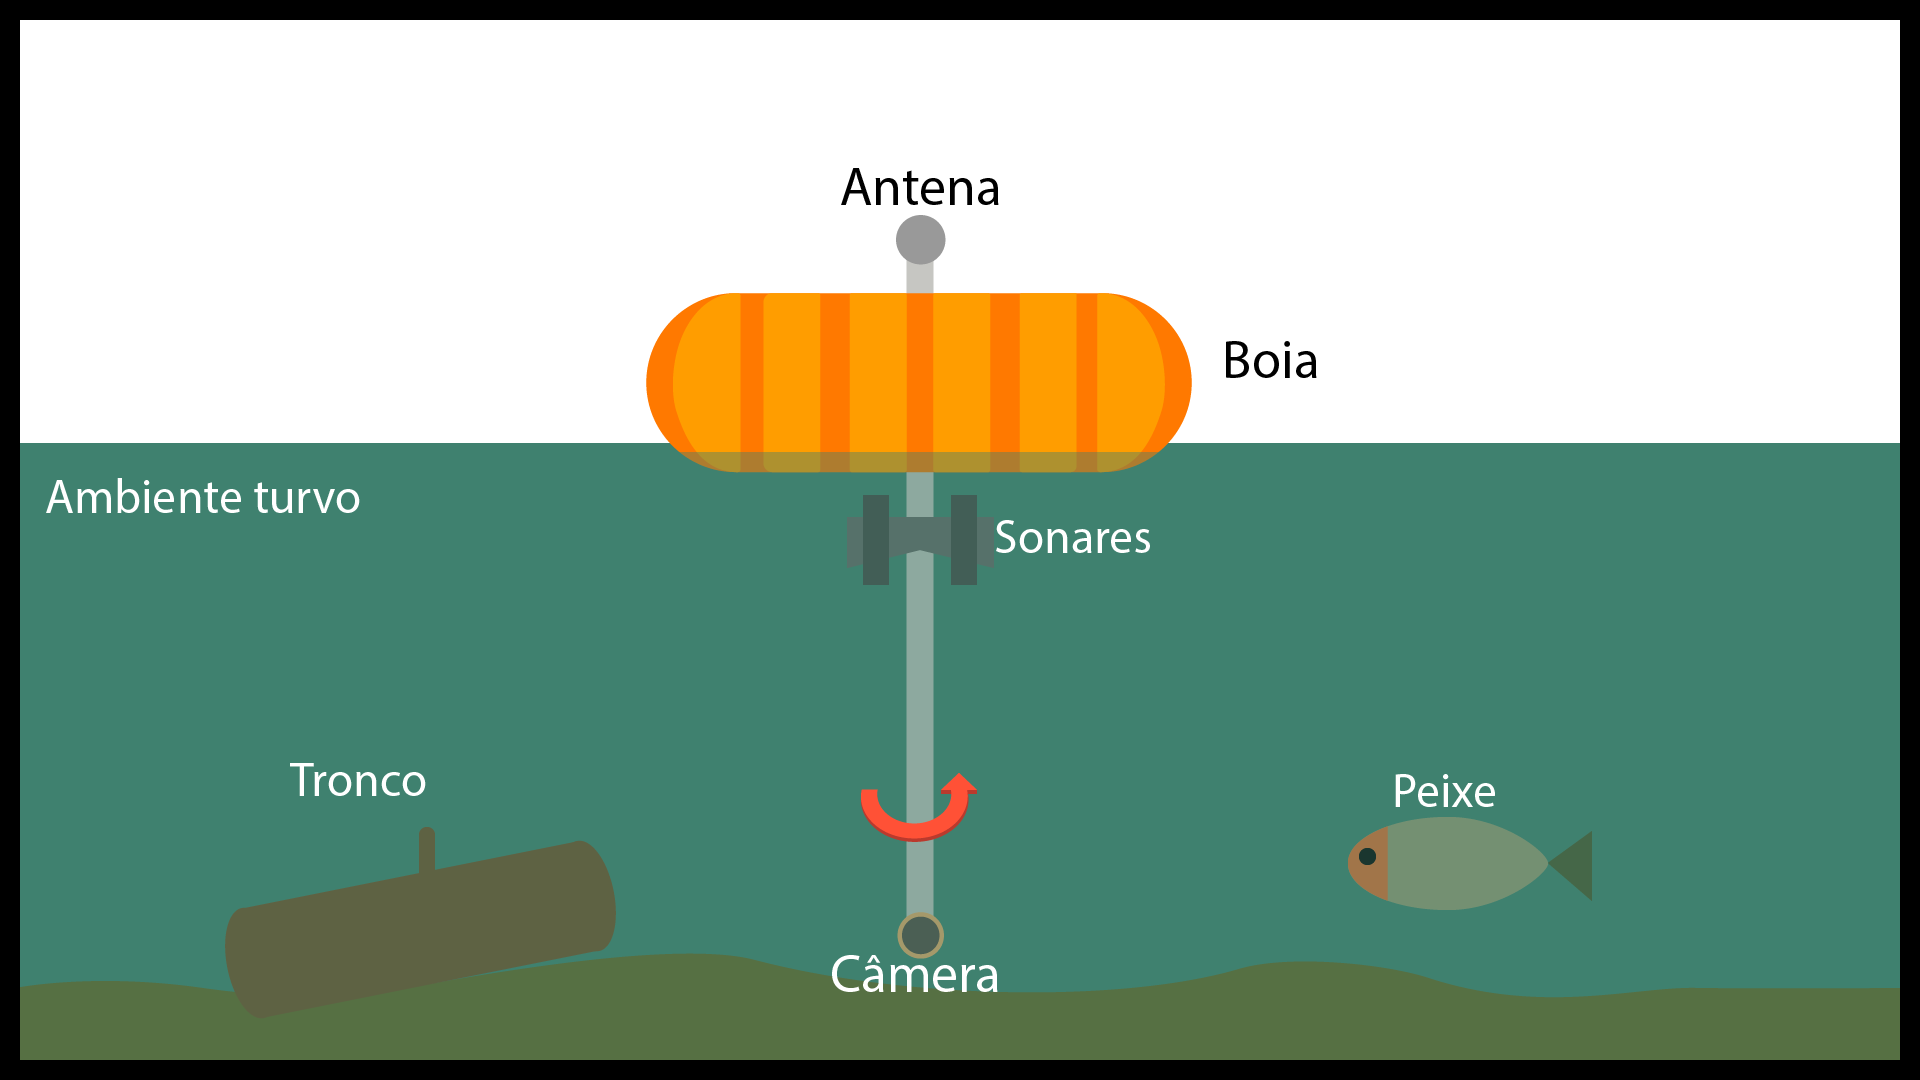
\includegraphics[width = 1\textwidth]			{resources/bigpicture}
    \legend{Fonte Própria}
\end{figure}
